\documentclass[12pt,a4paper]{proyectoinnovacion}
%------------------------------------------------------------------------------%
% INFORMACIÓN DEL ARTÍCULO Y METADATOS                                         %
%------------------------------------------------------------------------------%
\firstauthor{Rodolfo Arturo González Trillo}
\secondauthor{Carlos Oswaldo Alfaro Rodríguez}
\thirdauthor{}

\university{Universidad Internacional de La Rioja}
\school{Escuela Superior de Ingeniería y Tecnología}
\master{Maestría en Inteligencia Artificial}
\title{Sistema de visión artificial para monitoreo de mascotas}
\keywords{ia, unir, masctoas, monitoreo}
\date{\today}
%------------------------------------------------------------------------------%
% Metodologia, apendice.
\usepackage{pdflscape}

%Desarrollo conceptual.
\usepackage{animate}

% Apendice.
\usepackage{threeparttablex} % for "ThreePartTable" environment
\usepackage{array,multirow,graphicx}
\usepackage{float}
\usepackage{booktabs}

%Metodologia
\tikzset{every picture/.style={line width=0.75pt}} %set default line width to 0.75pt  

%Implementación
\usepackage{nicematrix} 

%%%%%%%%%%%%%%%%%%%%%%%%%%%%%%%%%%%%%%%%%%%%%%%%%%%%%%%%%%%%%%%%%%%%%%%%%%%%%%%%
\begin{document}

%------------------------------------------------------------------------------%
% Página de Título                                                             %
%------------------------------------------------------------------------------%
\maketitle

%------------------------------------------------------------------------------%
% Índice de contenidos                                                         %
%------------------------------------------------------------------------------%
{
  \setcounter{page}{2} 
  \hypersetup{linkcolor=black}
  \tableofcontents\thispagestyle{fancy}
}
\pagebreak

%------------------------------------------------------------------------------%
\section{Introducción}
%------------------------------------------------------------------------------%

En México, 7 de cada 10 hogares mexicanos tienen algún animal doméstico, y de estos, 89\% son perros \parencite{inegi2016}. Una gran parte de estas mascotas pasa su tiempo en solitario en sus viviendas, cuando sus dueños se marchan a realizar sus actividades laborales.

El vínculo que se forma entre una mascota y su amo puede llegar a ser muy profundo. Por esta razón, algunas mascotas y dueños pueden llegar a sentir ansiedad al separase de sus mascotas. En el caso de los perros, esta ansiedad se puede manifestar en comportamientos destructivos hacia los objetos de su hogar \parencite{parthasarathy2006}. 


\subsection{Justificación}
\label{sec:justificacion}

Este trabajo presenta una solución tecnológica para dos de los problemas causados por dejar a las mascotas en solitario:

\begin{enumerate}
  \item Disminuir la ansiedad de los dueños al dejar a su mascota sin vigilancia.
  \item Reducir o impedir el comportamiento destructivo cuando la mascota está en solitario. 
\end{enumerate}

Esta problemática se origina en las exigencias de los horarios laborales, en los que una persona promedio debe dedicar hasta 40 horas a la
semana de tiempo en la oficina. La ansiedad causada por la falta de atención y la soledad es la causa de los destrozos y malos comportamientos por parte de los animales \parencite{ibanes2022}.

Una solución que ha surgido para paliar este problema es el uso de paseadores. Sin embargo, el tiempo del paseo por lo regular no es mayor a una hora, por día. Insuficiente para la enorme cantidad de tiempo que los animales pasan en soledad día a día y además esto sólo es para los perros, ignorando a todo el grupo de los felinos.


\subsection{Objetivos}

De manera resumida, el presente trabajo plantea el uso de un sistema de visión artificial para monitorear la actividad de mascotas en tiempo real y reforzar ciertas pautas de entrenamiento, principalmente evitar la destrucción de mobiliario y el uso de este por parte de los animales. En la  \hyperref[sec:objetivos]{sección de objetivos se desarrollan más esta idea.}

\subsection{Estructura}

A continuación se hace una breve descripción de las secciones de este trabajo.

\begin{itemize}
  \item \hyperref[sec:objetivos]{Objetivos}. Se define cuál es el alcance del proyecto y los hitos que lo conforman. 
  \item \hyperref[sec:desarrolloconceptual]{Desarrollo conceptual}. Detalla el procedimiento y metodologías utilizadas para generar las ideas para el desarrollo del proyecto y cómo se llegó a la idea de la forma final del prototipo: un sistema que detecte el comportamiento simple de subirse a los muebles, que se pueda expandir a futuros comportamientos negativos.
  \item \hyperref[sec:metodologia]{Metodología}. Se describe la planificación y la metodología ágil que se usó a lo largo del proyecto SCRUM+LEAN+KANBAN. Los roles dentro del proyecto y las historias iniciales.
  \item \hyperref[sec:implementacion]{Implementación}. Cómo fueron los \textit{sprints} iniciales del proyecto y una descripción breve del desarrollo técnico. Además contiene posibles soluciones a contingencias.
  \item \hyperref[sec:validacion]{Validación}. Se mostró al usuario el resultado final del proyecto mediante una cámara usb conectada a una computadora y se preguntaron sus reflexiones acerca del sistema propuesto.
  \item \hyperref[sec:conclusiones]{Conclusiones y Trabajo Futuro}. Definen que se ha logrado con el proyecto y las futuras mejoras.
  \item \hyperref[ape:tablaencuesta]{Anexos}.
\end{itemize}



%------------------------------------------------------------------------------%
\section{Objetivos}
%------------------------------------------------------------------------------%

El objetivo del trabajo es:

\begin{quotebox}
  Probar que un sistema de vigilancia de mascotas que identifique de forma automática algunos comportamientos negativos es una propuesta viable.
\end{quotebox}


% Esta sección es el puente entre el estudio del dominio y la contribución a realizar. 

% Hay que definir el Objetivo Geneal (resumido en un par de líneas y explicar el qué, para qué y cómo se va a desarrollar la propuesta) y los Objetivos Específicos (suelen ser explicaciones de los diferentes pasos a seguir en la consecución del objetivo general)

% Para realizar este apartado, podrás apoyarte en los principios MELDS.
%------------------------------------------------------------------------------%
\section{Desarollo conceptual}
%------------------------------------------------------------------------------%
\label{sec:desarrolloconceptual}
Durante el desarrollo conceptual de este proyecto, se utilizó la metodología \textit{Design Thinking}, propuesto inicialmente por Larry Leifer \textcite{plattner2011}. Con el objetivo de obtener un proyecto bien planteado, basado en la retroalimentación de los usuarios finales se divide en las siguientes etapas:


\begin{itemize}
  \item Empatizar
  \item Definir
  \item Investigación de antecedentes
  \item Idear
  \item Prototipar: Cual será el prototipo que vas a utilizar
  \item Selección de prototipos y criterio para hacerlo  
\end{itemize}


%------------------------------------------------------------------------------%
\subsection{Empatizar}

Es la etapa inicial y se considera la más importante, pues las demás etapas se basan en esta. Se requiere conocer al cliente abordando sus verdaderas necesidades y haciéndolas propias. 

En el caso de este proyecto, esta etapa se realizó mediante la aplicación de un cuestionario a familiares, amigos y conocidos. Las preguntas ahondaban en el estado socioeconómica, la relación de los dueños con sus mascotas y sus ideas concretas sobre el problema planteado en la \hyperref[sec:justificacion]{justificación} del problema. Un resumen de las respuestas orginales se puede encontrar en el \hyperref[ape:tablaencuesta]{apéndice A}.


Se deduce de la encuesta que el usuario promedio de la aplicación son personas de entre 25 y 35 años con entre una y dos mascotas, con un salario entre 15,000 y 35,000 pesos mexicanos, viven en departamentos o casas sin patio, adicionalmente trabajan 40 horas a la semana y realizan actividades fuera de su casa lo que les impide cuidar a su mascota durante gran parte del día. Así mismo el usuario tiene la capacidad de acceder a una cámara web desde su laptop o computadora y deben ser nativos digitales cómodos con el uso de aplicaciones web.

Así mismo el usuario ve a las mascotas como parte importante de su núcleo familiar, no como un elemento de guardia o de servicio. Parte de ver a sus mascotas como parte de su núcleo familiar genera preocupación al dejarlo sin supervisión, especialmente por situaciones que lo pudieran poner en peligro, como el que tire algún objeto y se lastime, independientemente del costo material que pudiera ocasionar.

Con los datos de la encuesta (\hyperref[ape:tablaencuesta]{apéndice A}) también se realizó el mapa de empatía de la \figura{fig:mapaempatia}. 


\begin{landscape}
  \begin{figure}
      \centering
      \caption[Mapa de empatía del proyecto.]{Mapa de empatía realizado con los resultados. Cada sección de la figura corresponde a distintas experiencias sensoriales y emocionales acerca del problema a trata. Los esfuerzos representa lo que el usuario final está dispuesto a hacer para resolver el problema y los resultados lo que espera lograr.}
      \label{fig:mapaempatia}
      \includegraphics[width=\linewidth]{mapa_empatia.pdf}
  \end{figure}
\end{landscape}

%------------------------------------------------------------------------------%
\subsection{Definir}
\label{sec:definir}

En esta etapa se identificaron las necesidades principales. Luego de la encuesta y el mapa de empatía (\figura{fig:mapaempatia}) es fácil ver que las necesidades principales son:


\begin{itemize}
  \item Una manera de mantener a la mascota vigilada para que no se haga daño.\item Disminuir el comportamiento destructivo cuando la mascota abandona la casa.
\end{itemize}

%------------------------------------------------------------------------------%
\subsection{Idear}
\label{sec:idear}

Consiste en pensar en distintas soluciones a los problemas de la \hyperref[sec:definir]{etapa de definición}.

Se llegó al conceso de que una cámara, conectada a una aplicación que transmita en tiempo real a las mascotas, es la solución a los problemas de vigilancia. Para el problema de disminuir el comportamiento destructivo se pensó en distintas soluciones que analicen el video en tiempo real y de forma automática, notifiquen y/o emitan una alerta al dueño de la mascota cuando esta :

\begin{itemize}
  \item está arriba de los muebles o en zonas indebidas.
  \item destruye objetos, como calzado o sandalias.
  \item está ladrando o aullando en exceso.
  \item se pelea con otras mascotas.
\end{itemize}

Luego de cierta deliberación, se determinó que el la detección automática de  comportamiento negativo más factible a programar dentro de las limitaciones de tiempo es el problema de cuando la mascota está en zonas indebidas, concretamente arriba de muebles. Los otros problemas quedarán pendientes para futuras iteraciones de este proyecto.

%------------------------------------------------------------------------------%
\subsection{Prototipar}

En esta etapa, se realiza un prototipo de la solución, que se mostrará más tarde a los encuestados.


Realizar una aplicación que envía video real a través de la nube no es novedoso. Detectar comportamientos inusuales de forma automática en las mascotas sí. Es por eso que se decidió que para el prototipo lo primero que se tenía que pensar es cómo ésto era factible. 

Se decidió que para el alcance del proyecto lo ideal era identificar sólo un comportamiento negativo. Luego de una investigación exhaustiva y cualitativa en Google y Youtube se verificó que una gran parte de los problemas de mal comportamiento en mascotas es la destrucción de muebles. En  una gran parte de estos vídeos la mascota destruye el mueble desde arriba del mismo. Si se detecta cuando la mascota se sube a un mueble, se puede evitar la destrucción en una buena parte de los casos. Se propone un programa que actúe como el de \figura{fig:mascotas}.


\begin{figure}
  \centering
  \caption[Proceso de identificación ]{Proceso de detección de la mascota cuando está sobre los muebles en tiempo real:  La entrada (en la parte superior) es una secuencia de vídeo. Esta secuencia en video puede ser un fragmento de unos cuantos cuadros del vídeo en tiempo real.  Dos procesos ocurren de forma semi simultánea. \textit{Procesar el fondo}: Luego de varios cuadros estáticos, se determinan las partes de la imagen que no están en movimiento. Con una red de segmentación automática, se segmenta la imgagen y se detecta el suelo. \textit{Procesar objetos en movimiento}: Se contrastan los objetos que difieren del fondo, se detectan sus fronteras, y se determina si se trata de una mascota o no. Se detecta la probabilidad de estar fuera del suelo. Si esta probabilidad es alta por varios segundos, se emite la alerta.}
  \label{fig:mascotas}
  \includegraphics[width=\columnwidth]{mascotas.pdf}
\end{figure}


A partir del diagrama del proceso de detección, se realizó una animación de cómo funcionaría la aplicación en su versión final (\figura{fig:animacion}).

\begin{figure}
  \centering
  \caption[Prototipo del proyecto final.]{Protipo del proyecto final. Requiere \textit{Acrobat Reader}, \textit{KDE Okular}, \textit{PDF-XChange} o \textit{Foxit Reader} para  visualizar, de lo contrario puede verse en el archivo \textit{.gif} adjunto a este documento.}
  \animategraphics[controls,autoplay,width=0.5\columnwidth]{12}{gif/e05a1b6f887641509ed0d893e0d9609aEX3IJwYFFaSk4UUz-}{0}{84}
  \label{fig:animacion}
\end{figure}


%------------------------------------------------------------------------------%
\subsection{Evaluar}

El video prototipo de la \figura{fig:animacion} fue mostrado a los usuarios que habían respondido las preguntas de la primera encuesta. Los comentarios mostrados fueron positivos, destacando que esta función de detección de animales sobre los muebles ``sería de gran utilidad'' y ``estarían dispuestos a pagar por ella.''. Algunos sugirieron añadir características como conexión con servicios de paseo o cuidado de mascotas, monitoreo de estrés, monitoreo de ejercicio. Estas soluciones se tendrán en cuenta para mejoras futuras.

\newlength{\lanscapetablewidth}
\setlength{\lanscapetablewidth}{1.3\linewidth}
%------------------------------------------------------------------------------%
\section{Metodología}
%------------------------------------------------------------------------------%
\label{sec:metodologia}


Se ha usado una metodología ágil híbrida para el desarrollo del proyecto de SCRUM, LEAN y KANBAN.  

Las metodologías ágiles permiten un desarrollo incremental. Sus principales
características es que se apoyan en los individuos e interacciones y le dan preferencia a versiones ejecutables desde el inicio del proyecto, que se van incrementando de forma iterativa \parencite{pmi2017}. 

SCRUM es una metodología orientada al desarrollo de software en equipos pequeños, idealmente de hasta 10 personas. Se caracteriza son los llamados \textit{sprints}, los cuales consisten en tareas asignadas a etapas de usualmente dos semanas y la estructura de los roles que se sigue en este proyecto \parencite{schwaber2020}.

KANBAN es un sistema de organización de tareas que se utiliza junto con SCRUM en el cual las tareas suelen escribirse en tarjetas agrupadas en categorías de acuerdo al estado de la tarea —en proceso, por planificar, terminado, etc— cuando se combina con SCRUM se suele escribir el sprint al cual pertenecen las tareas. Las tarjetas suelen ser virtuales \parencite{stellman2014}. 

LEAN es un marco de valores que promueve ``la organización de las actividades humanas para entregar más beneficios a la sociedad y al individuo, eliminando los despilfarros'' \parencite{womack2003}. En la \figura{fig:penasmientolean} se describe un poco estos valores.

\begin{figure}
    \centering
    \caption[Pensamiento LEAN]{Valores LEAN en el desarollo de software: \textit{1. Eliminar el despilfarro} evitar requerimientos procesos y funciones innecesarias, cambiar equipo, etc. \textit{2. Ampliar el aprendizaje} dedicar recursos a la mejora de las habilidades. \textit{3. Posponer decisiones} así se evitan discusiones largas y pérdidas de tiempo. \textit{4. Liberar pronto} versiones para poder tener retroalimentación de los usuarios y el cliente. \textit{5. Empoderar al equipo} promocionar la autonomía, asumir que todos saben hacer su trabajo. \textit{6. Construir calidad} debe ser el corazón del proyecto de inicio a fin. \textit{7. Optimizar el sistema} implementar métodos de medición para optimizar procesos en cada iteración.}
    \label{fig:penasmientolean}
    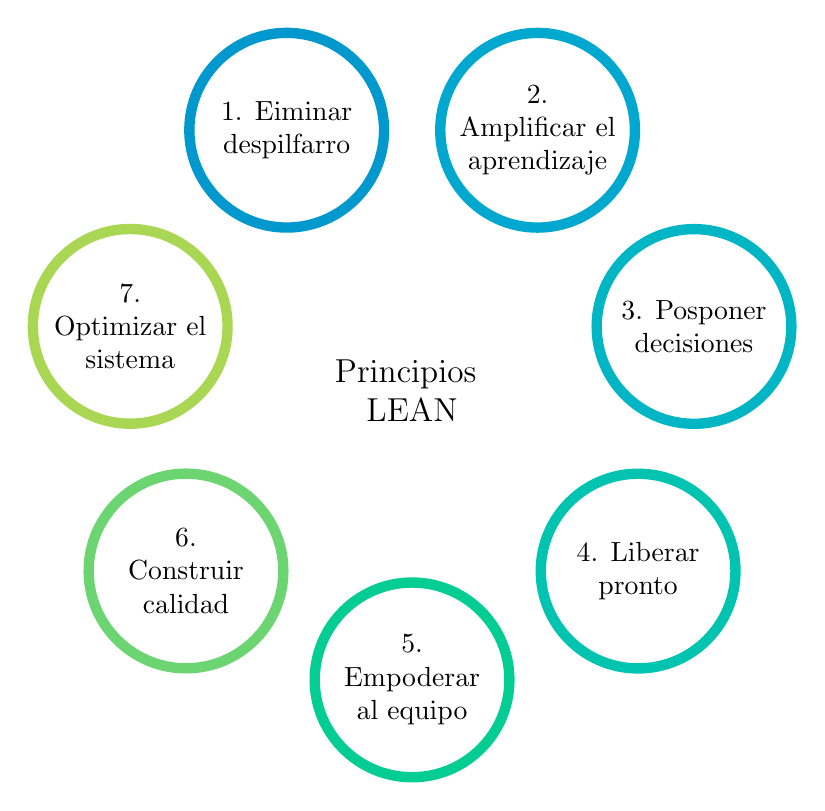
\begin{tikzpicture}[x=0.75pt,y=0.75pt,yscale=-1,xscale=1]
%uncomment if require: \path (0,399); %set diagram left start at 0, and has height of 399

%Flowchart: Connector [id:dp6671534120935239] 
\draw  [color={rgb, 255:red, 0; green, 152; blue, 205 }  ,draw opacity=1 ][line width=3.75]  (192.38,68.52) .. controls (192.38,42.62) and (213.38,21.62) .. (239.29,21.62) .. controls (265.19,21.62) and (286.19,42.62) .. (286.19,68.52) .. controls (286.19,94.42) and (265.19,115.42) .. (239.29,115.42) .. controls (213.38,115.42) and (192.38,94.42) .. (192.38,68.52) -- cycle ;
%Flowchart: Connector [id:dp9742464437933368] 
\draw  [color={rgb, 255:red, 0; green, 168; blue, 207 }  ,draw opacity=1 ][line width=3.75]  (313.27,68.54) .. controls (313.27,42.64) and (334.27,21.64) .. (360.17,21.64) .. controls (386.08,21.64) and (407.07,42.64) .. (407.07,68.54) .. controls (407.07,94.45) and (386.08,115.44) .. (360.17,115.44) .. controls (334.27,115.44) and (313.27,94.45) .. (313.27,68.54) -- cycle ;
%Flowchart: Connector [id:dp17986667998434147] 
\draw  [color={rgb, 255:red, 0; green, 182; blue, 197 }  ,draw opacity=1 ][line width=3.75]  (388.63,163.07) .. controls (388.63,137.17) and (409.63,116.17) .. (435.53,116.17) .. controls (461.43,116.17) and (482.43,137.17) .. (482.43,163.07) .. controls (482.43,188.97) and (461.43,209.97) .. (435.53,209.97) .. controls (409.63,209.97) and (388.63,188.97) .. (388.63,163.07) -- cycle ;
%Flowchart: Connector [id:dp49064716171042055] 
\draw  [color={rgb, 255:red, 0; green, 195; blue, 176 }  ,draw opacity=1 ][line width=3.75]  (361.7,280.92) .. controls (361.7,255.02) and (382.7,234.02) .. (408.6,234.02) .. controls (434.51,234.02) and (455.5,255.02) .. (455.5,280.92) .. controls (455.5,306.83) and (434.51,327.83) .. (408.6,327.83) .. controls (382.7,327.83) and (361.7,306.83) .. (361.7,280.92) -- cycle ;
%Flowchart: Connector [id:dp4374690028497701] 
\draw  [color={rgb, 255:red, 4; green, 205; blue, 147 }  ,draw opacity=1 ][line width=3.75]  (252.78,333.35) .. controls (252.78,307.45) and (273.77,286.45) .. (299.68,286.45) .. controls (325.58,286.45) and (346.58,307.45) .. (346.58,333.35) .. controls (346.58,359.26) and (325.58,380.25) .. (299.68,380.25) .. controls (273.77,380.25) and (252.78,359.26) .. (252.78,333.35) -- cycle ;
%Flowchart: Connector [id:dp9167083401815027] 
\draw  [color={rgb, 255:red, 109; green, 212; blue, 114 }  ,draw opacity=1 ][line width=3.75]  (143.87,280.88) .. controls (143.87,254.98) and (164.87,233.98) .. (190.77,233.98) .. controls (216.67,233.98) and (237.67,254.98) .. (237.67,280.88) .. controls (237.67,306.78) and (216.67,327.78) .. (190.77,327.78) .. controls (164.87,327.78) and (143.87,306.78) .. (143.87,280.88) -- cycle ;
%Flowchart: Connector [id:dp24671509877720965] 
\draw  [color={rgb, 255:red, 169; green, 215; blue, 83 }  ,draw opacity=1 ][line width=3.75]  (116.99,163.02) .. controls (116.99,137.12) and (137.99,116.12) .. (163.89,116.12) .. controls (189.8,116.12) and (210.79,137.12) .. (210.79,163.02) .. controls (210.79,188.92) and (189.8,209.92) .. (163.89,209.92) .. controls (137.99,209.92) and (116.99,188.92) .. (116.99,163.02) -- cycle ;

% Text Node
\draw (239.29,68.52) node   [align=left] {\begin{minipage}[lt]{54.92pt}\setlength\topsep{0pt}
\begin{center}
1. Eiminar\\despilfarro
\end{center}

\end{minipage}};
% Text Node
\draw (360.17,68.54) node   [align=left] {\begin{minipage}[lt]{58.29pt}\setlength\topsep{0pt}
\begin{center}
2. \\Amplificar el\\aprendizaje
\end{center}

\end{minipage}};
% Text Node
\draw (435.53,163.07) node   [align=left] {\begin{minipage}[lt]{57.75pt}\setlength\topsep{0pt}
\begin{center}
3. Posponer\\decisiones
\end{center}

\end{minipage}};
% Text Node
\draw (408.6,280.92) node   [align=left] {\begin{minipage}[lt]{48.68pt}\setlength\topsep{0pt}
\begin{center}
4. Liberar \\pronto
\end{center}

\end{minipage}};
% Text Node
\draw (299.68,333.35) node   [align=left] {\begin{minipage}[lt]{53.21pt}\setlength\topsep{0pt}
\begin{center}
5.\\Empoderar\\al equipo
\end{center}

\end{minipage}};
% Text Node
\draw (190.77,280.88) node   [align=left] {\begin{minipage}[lt]{46.95pt}\setlength\topsep{0pt}
\begin{center}
6.\\Construir \\calidad
\end{center}

\end{minipage}};
% Text Node
\draw (163.89,163.02) node   [align=left] {\begin{minipage}[lt]{57.15pt}\setlength\topsep{0pt}
\begin{center}
7.\\Optimizar el\\sistema
\end{center}

\end{minipage}};
% Text Node
\draw (299.7,194.04) node  [font=\large] [align=left] {\begin{minipage}[lt]{55.79pt}\setlength\topsep{0pt}
Principios
\begin{center}
LEAN
\end{center}

\end{minipage}};


\end{tikzpicture}

    \source{Elaboración propia con información de \figurecite{ferreit2021}.}
  \end{figure}
  

\subsection{Roles}

Los roles del proyecto están asignados de acuerdo a la metodología SCRUM. Debido a lo pequeño del equipo de trabajo los autores ocupan varios de los roles.

\begin{itemize}
  \item \textit{Product Owner} Responsable de maximizar el valor del producto final: \atsecondauthor.
  \item \textit{Scrum Master} Encargado de la planificación y el entendimiento de la metodología SCRUM: \atfirstauthor
  \item \textit{Development Team Mebers}: Ambos autores.
\end{itemize}


\subsection{\textit{Sprints}}
\label{sec:sprints}

Se definió que la duración de cada \textit{sprint} para este proyecto fuera de una semana. Un \textit{sprint} consta de las siguientes ceremonias:


\begin{itemize}
  \item Planificación: se define que se hará durante el \textit{sprint} — 1 hora al inicio del mismo.
  \item Implementación: el trabajo en si mismo —3 días de trabajo, y 1 día de pruebas, con un día liberación.  
  \item Demostración y revisión —se presenta el trabajo y se presentan comentarios y partes a corregir —reunión de 1 hora.
  \item Retrospectiva: se presenta una versión del trabajo con correcciones —reunión de 1 hora. 
  \item Refinamiento: revisión de historias existentes, adición de nuevas historias.
\end{itemize}


\subsection{\textit{Historias Iniciales}}

Las historias se definieron en Azure. Se pueden consultar a detalle en \href{https://dev.azure.com/petartificialvision}{petartificialvision}. Aquí presentamos una tabla con las historias.

\begin{landscape}
    \begin{small}
    \begin{longtable}{
        p{0.04\lanscapetablewidth}p{0.11\lanscapetablewidth}p{0.18\lanscapetablewidth}p{0.36\lanscapetablewidth}p{0.07\lanscapetablewidth}p{0.14\lanscapetablewidth}p{0.11\lanscapetablewidth}
    }
        \caption{Historias iniciales del proyecto.}\label{tab:historias}\\
        \toprule
        ID &
        Tipo de historia &
        Título &
        Descripción &
        Puntos de esfuerzo &
        Asignado a &
        Estado \\
        \midrule
        \endfirsthead
        \caption*{\textbf{\textup{Tabla \ref*{tab:historias} Continuación.}}  Historias iniciales del proyecto.}\\
        \toprule
        ID &
        Tipo de historia &
        Título &
        Descripción &
        Puntos de esfuerzo &
        Asignado a &
        Estado \\
        \midrule        
        \endhead
        \midrule\multicolumn{7}{r}{\itshape Continua en la siguiente página.}\\\endfoot
        \bottomrule\endlastfoot
        2 &
        Tarea &
        Entrevistar usuarios &
        Como product owner quiero aplicar la entrevista creada en la tarea Tarea 10: Diseñar entrevista para obtener retroalimentación para usuarios. - Boards (azure.com) a al menos 15 posibles usuarios de la aplicación. &
        7 &
        \atfirstauthor &
        Terminado \\
        4 &
        Tarea &
        Desarrollar código para acceder a la camara. &
        Como desarrollador quiero crear un segmento de código que me permita acceder a una camára web (si el dispositivo la tiene) desde un programa de python, una vez que se acceda a la camára quiero poder pasar el vídeo desde la camára a otros segmentos de código. &
        11 &
        \atfirstauthor &
        Por Hacer \\
        6 &
        Tarea &
        Entrenar red neuronal para segmentación de imágenes. &
        Como desarrollador quiero entrenar la red neuronal seleccionada en  para segmentar automáticamente imágenes. &
        17 &
        \atsecondauthor &
        Por Hacer \\
        7 &
        Tarea &
        Desarrollar detector de movimiento &
        Como desarrollador quiero crear un segmento de código que permita detectar movimiento en un segmento de vídeo.  &
        13 &
        \atfirstauthor &
        Por Hacer \\
        10 &
        Tarea &
        Diseñar entrevista para obtener retroalimentación para usuarios. &
        Yo como product owner quiero diseñar una entrevista que me permita obtener retroalimentación de los usuarios, está entrevista debe estar publicada en google forms para que los usuarios puedan acceder fácilmente a ella. &
        5 &
        \atfirstauthor &
        Terminado \\
        11 &
        Tarea &
        Entrevistar Usuarios. &
        {} &
        {} &
        \atfirstauthor &
        Por Hacer \\
        12 &
        Tarea &
        Investigar opciones para la segmentación de imágenes. &
        Yo como desarrollador quiero investigar las posibles opciones existentes para realizar segmentación de imágenes automática. Debo recabar las posibles opciones y presentarlas en la reunión de refinamiento del siguiente sprint (una vez terminada esta historia). &
        5 &
        \atsecondauthor &
        Por Hacer \\
        18 &
        Tarea &
        Detección de suelos. &
        Como desarrollador quiero desarrollar una red neuronal y entrenarla para detectar suelos. &
        17 &
        \atsecondauthor &
        Terminado \\
    \end{longtable} 
\end{small}
\end{landscape}


\subsection{Gestión de historias}

Se ha ocupado Azure Devops debido a su integración con GiHub y su amplio abanico de herramientas gratuitas para la administración de equipos, así mismo tiene una excelente integración con todo el ecosistema Microsoft.

\subsection{Puntos de esfuerzo}

Los puntos de esfuerzo se han asignado a cada historia ocupando el modelo de números primos, donde el esfuerzo de una historia se mide usando números primos, lo que provoca que el crecimiento de esfuerzo no sea lineal y permite observar mejor si una historia debe ser dividida o simplificada al tener esfuerzos muy grandes.

\subsection{Etapas LEAN}

Las etapas del inicio de un proyecto siguiendo los principios LEAN son las siguientes \parencite{cardenas}.

\subsubsection{Propón una hipótesis}

Esta etapa esta relacionada con el objetivo del trabajo \hyperref[sec:objetivos]{objetivo del trabajo}, que se puede escribir en forma de hipótesis como:

\begin{quotebox}
Hay personas dispuestas a comprar un sistema inteligente de vigilancia de mascotas.
\end{quotebox}

\subsubsection{Valida la hipótesis}

Se realizó en parte en el \hyperref[sec:desarrolloconceptual]{desarollo conceptual}. La hipótesis se validó con un prototipo que fue mostrado al público. La hipótesis se seguirá verificando mostrando y obteniendo la retroalimentación de los usuarios.

\subsubsection{Mide la hipótesis}

Esta etapa se explica en la \seccion{sec:mediciones}.

\subsubsection{Aprende del proceso}

Dentro de LEAN, se pide mejorar el proceso con la retroalimentación de los clientes, incluso cambiar la hipótesis. Esto será vital durante el desarrollo del proyecto.

\subsection{Mediciones}
\label{sec:mediciones}

Las mediciones se harán al inicio de cada \textit{sprint}. Para medir la calidad se establecerá un esfuerzo objetivo que se contrastará con la evaluación de capacidad real al final de cada \textit{sprint} y la cantidad de \textit{bugs} introducidos con cada historia para tener una idea de la mejora en la calidad del software conforme pasen los \textit{sprints}.

También se utilizarán KPI's informativos durante el proyecto de estimación de ventas y retorno de inversión, y algunos relacionados a la distribución de la aplicación en Google Store, como las evaluaciones, la calificación y la popularidad.











%------------------------------------------------------------------------------%
\section{Implementación de la propuesta}
%------------------------------------------------------------------------------%

\subsection{Planificación y estimación}

\begin{table}
	\small\centering
    \caption{Cronograma y planificación de los \textit{sprints}. La ``S'' es de \textit{sprint}.}
    \label{tab:sprints}
    \begin{NiceTabular}{p{4.5cm}|c|c|c|c|c|c|c|c|c|c|c|c|c}[
        code-before = 
        \cellcolor{mygreen}{2-2, 2-3, 2-8, 2-11}
        \cellcolor{mygreen}{3-2, 3-3, 3-8, 3-11}
        \rectanglecolor{mygreen}{4-4}{4-6}
        \rectanglecolor{mygreen}{5-4}{5-7}\rectanglecolor{mygreen}{5-9}{5-13}
        \cellcolor{mygreen}{6-8, 6-11}
        \rectanglecolor{mygreen}{7-4}{7-13}
        \rectanglecolor{mygreen}{8-7}{8-13}
        \cellcolor{mygreen}{9-7, 9-10, 9-13}
     ]
        \hline
        Actividad                  & S1& S2& S3& S4& S5& S6& S7& S8& S9&S10&S11&S12\\
        \hline
        Investigación del producto &   &   &   &   &   &   &   &   &   &   &   &   \\
        \hline
        Diseño                     &   &   &   &   &   &   &   &   &   &   &   &   \\
        \hline
        Desarrollo red neuronal    &   &   &   &   &   &   &   &   &   &   &   &   \\
        \hline
        Desarrollo aplicación web  &   &   &   &   &   &   &   &   &   &   &   &   \\
        \hline
        Retroalimentación          &   &   &   &   &   &   &   &   &   &   &   &   \\
        \hline
        Desarrollo 
        API             &   &   &   &   &   &   &   &   &   &   &   &   \\
        \hline
        Entrenamiento y mejora red neuronal &   &   &   &   &   &   &   &   &   &   &   \\
        \hline
        Lanzamiento PMV            &   &   &   &   &   &   &   &   &   &   &   &   \\
        \hline      
    \end{NiceTabular}
\end{table}



\begin{table}
    \small\centering
    \caption{Costos del proyecto.}
    \label{tab:costos}
    \begin{tabular}{p{4.5cm}rrrr}
        \toprule
        Recursos Humanos & Cantidad & Costo mensual & Meses & Subtotal \\
        \midrule
        \textit{Senior FullStack Developer} & 1 & 50,000 & 3 & 150,000 \\
        \textit{Junior Fullstack Developer} & 1 & 28,000 & 3 & 84,000 \\
        \textit{Senior Ux Design}er & 1 & 35,000 & 3 & 105,000 \\
        Arquitecto de sistemas \textit{Cloud mid level} & 1 & 75,000 & 3 & 225,000 \\
        \textit{Product Owner }& 1 & 65,000 & 3 & 195,000 \\
        \midrule
        &  &  &  Total & 759,000 \\
        \bottomrule
        \toprule
        Servicios & Cantidad & Costo mensual & Meses & Subtotal \\
        \midrule
        Servicios Azure & 1 & 51,413 & 3 & 154,240 \\
        \midrule
        &  &  &  Total & 154,240 \\
        \bottomrule
        \toprule 
        Materiales & & Cantidad & Costo & Subtotal \\
        \midrule
        \textit{Laptop hp zbook 14 Firefly G8} & & 4 & 35,000 & 140,000 \\
        \textit{Macbook Pro MKGP3E/A} & & 2 & 49,000 & 98,000 \\
        \midrule
        &  &  Total &  & 238,000 \\
        \bottomrule 
        \toprule 
        Infraestructura &  & Costo mensual & Meses & Subtotal \\
        \midrule
        Internet & & 3,000 & 14 & 42,000 \\
        \midrule
        &  &  Total &  & 42,000 \\
        \bottomrule
        \toprule 
        \multicolumn{4}{r}{\textbf{Total global del proyecto}} & \textbf{1,193,240} \\
        \bottomrule
    \end{tabular}
\end{table}

\subsection{Prototipo}

\begin{figure}
    \centering
    \caption[Diagrama del funcionamiento de la aplicación.]{Diagrama del funcionamiento de la aplicación.}
    \label{fig:funcionamiento}
    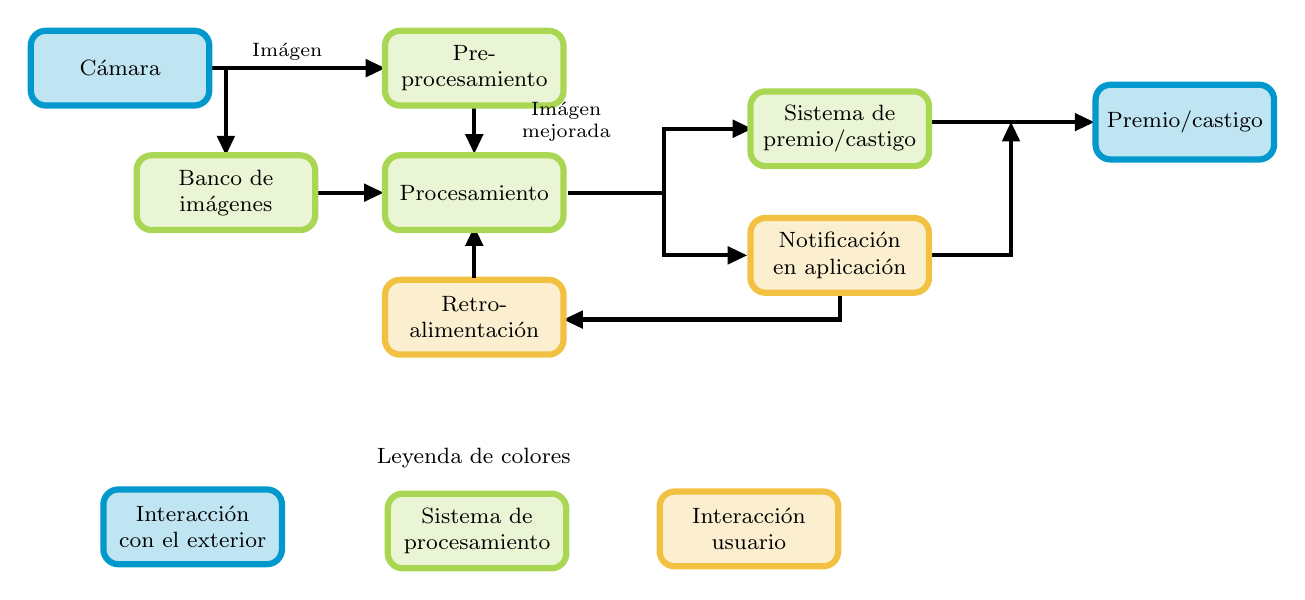
\begin{tikzpicture}[x=0.75pt,y=0.75pt,yscale=-1,xscale=1]
%uncomment if require: \path (0,480); %set diagram left start at 0, and has height of 480

%Straight Lines [id:da49883994500921447] 
\draw [line width=1.5]    (296.67,97.67) -- (343.07,97.67) -- (343.07,127.87) -- (379.07,127.87) ;
\draw [shift={(383.07,127.87)}, rotate = 180] [fill={rgb, 255:red, 0; green, 0; blue, 0 }  ][line width=0.08]  [draw opacity=0] (9.29,-4.46) -- (0,0) -- (9.29,4.46) -- cycle    ;
%Straight Lines [id:da2905724578829102] 
\draw [line width=1.5]    (296.67,97.67) -- (343.07,97.67) -- (343.07,66.87) -- (381.47,66.87) ;
\draw [shift={(385.47,66.87)}, rotate = 180] [fill={rgb, 255:red, 0; green, 0; blue, 0 }  ][line width=0.08]  [draw opacity=0] (9.29,-4.46) -- (0,0) -- (9.29,4.46) -- cycle    ;
%Straight Lines [id:da10483512115459537] 
\draw [line width=1.5]    (124.67,37.67) -- (204.67,37.67) ;
\draw [shift={(208.67,37.67)}, rotate = 180] [fill={rgb, 255:red, 0; green, 0; blue, 0 }  ][line width=0.08]  [draw opacity=0] (9.29,-4.46) -- (0,0) -- (9.29,4.46) -- cycle    ;
%Straight Lines [id:da4860403173310909] 
\draw [line width=1.5]    (175.87,97.67) -- (203.87,97.67) ;
\draw [shift={(207.87,97.67)}, rotate = 180] [fill={rgb, 255:red, 0; green, 0; blue, 0 }  ][line width=0.08]  [draw opacity=0] (9.29,-4.46) -- (0,0) -- (9.29,4.46) -- cycle    ;
%Straight Lines [id:da39629635865875956] 
\draw [line width=1.5]    (469.47,63.67) -- (546.27,63.67) ;
\draw [shift={(550.27,63.67)}, rotate = 180] [fill={rgb, 255:red, 0; green, 0; blue, 0 }  ][line width=0.08]  [draw opacity=0] (9.29,-4.46) -- (0,0) -- (9.29,4.46) -- cycle    ;
%Straight Lines [id:da6360560713651083] 
\draw [line width=1.5]    (343.07,66.87) -- (385.47,66.87) ;
%Straight Lines [id:da7217883827854481] 
\draw [line width=1.5]    (470.27,127.87) -- (510.27,127.87) -- (510.27,67.67) ;
\draw [shift={(510.27,63.67)}, rotate = 90] [fill={rgb, 255:red, 0; green, 0; blue, 0 }  ][line width=0.08]  [draw opacity=0] (9.29,-4.46) -- (0,0) -- (9.29,4.46) -- cycle    ;
%Straight Lines [id:da9212509405858289] 
\draw [line width=1.5]    (427.74,145.47) -- (427.74,158.8) -- (298.67,158.8) ;
\draw [shift={(294.67,158.8)}, rotate = 360] [fill={rgb, 255:red, 0; green, 0; blue, 0 }  ][line width=0.08]  [draw opacity=0] (9.29,-4.46) -- (0,0) -- (9.29,4.46) -- cycle    ;
%Straight Lines [id:da7493384106097625] 
\draw [line width=1.5]    (132,38.8) -- (132,75.6) ;
\draw [shift={(132,79.6)}, rotate = 270] [fill={rgb, 255:red, 0; green, 0; blue, 0 }  ][line width=0.08]  [draw opacity=0] (9.29,-4.46) -- (0,0) -- (9.29,4.46) -- cycle    ;
%Rounded Rect [id:dp5515000815065423] 
\draw  [color={rgb, 255:red, 0; green, 152; blue, 205 }  ,draw opacity=1 ][fill={rgb, 255:red, 0; green, 152; blue, 205 }  ,fill opacity=0.25 ][line width=2.25]  (38,26.87) .. controls (38,22.89) and (41.22,19.67) .. (45.2,19.67) -- (116.8,19.67) .. controls (120.78,19.67) and (124,22.89) .. (124,26.87) -- (124,48.47) .. controls (124,52.44) and (120.78,55.67) .. (116.8,55.67) -- (45.2,55.67) .. controls (41.22,55.67) and (38,52.44) .. (38,48.47) -- cycle ;
%Rounded Rect [id:dp32085170046138056] 
\draw  [color={rgb, 255:red, 0; green, 152; blue, 205 }  ,draw opacity=1 ][fill={rgb, 255:red, 0; green, 152; blue, 205 }  ,fill opacity=0.25 ][line width=2.25]  (73,247.87) .. controls (73,243.89) and (76.22,240.67) .. (80.2,240.67) -- (151.8,240.67) .. controls (155.78,240.67) and (159,243.89) .. (159,247.87) -- (159,269.47) .. controls (159,273.44) and (155.78,276.67) .. (151.8,276.67) -- (80.2,276.67) .. controls (76.22,276.67) and (73,273.44) .. (73,269.47) -- cycle ;
%Rounded Rect [id:dp20895200609973108] 
\draw  [color={rgb, 255:red, 0; green, 152; blue, 205 }  ,draw opacity=1 ][fill={rgb, 255:red, 0; green, 152; blue, 205 }  ,fill opacity=0.25 ][line width=2.25]  (551,52.87) .. controls (551,48.89) and (554.22,45.67) .. (558.2,45.67) -- (629.8,45.67) .. controls (633.78,45.67) and (637,48.89) .. (637,52.87) -- (637,74.47) .. controls (637,78.44) and (633.78,81.67) .. (629.8,81.67) -- (558.2,81.67) .. controls (554.22,81.67) and (551,78.44) .. (551,74.47) -- cycle ;
%Rounded Rect [id:dp8032697712302126] 
\draw  [color={rgb, 255:red, 169; green, 215; blue, 83 }  ,draw opacity=1 ][fill={rgb, 255:red, 169; green, 215; blue, 83 }  ,fill opacity=0.25 ][line width=2.25]  (210,249.87) .. controls (210,245.89) and (213.22,242.67) .. (217.2,242.67) -- (288.8,242.67) .. controls (292.78,242.67) and (296,245.89) .. (296,249.87) -- (296,271.47) .. controls (296,275.44) and (292.78,278.67) .. (288.8,278.67) -- (217.2,278.67) .. controls (213.22,278.67) and (210,275.44) .. (210,271.47) -- cycle ;
%Rounded Rect [id:dp33703696522885096] 
\draw  [color={rgb, 255:red, 169; green, 215; blue, 83 }  ,draw opacity=1 ][fill={rgb, 255:red, 169; green, 215; blue, 83 }  ,fill opacity=0.25 ][line width=2.25]  (89,86.87) .. controls (89,82.89) and (92.22,79.67) .. (96.2,79.67) -- (167.8,79.67) .. controls (171.78,79.67) and (175,82.89) .. (175,86.87) -- (175,108.47) .. controls (175,112.44) and (171.78,115.67) .. (167.8,115.67) -- (96.2,115.67) .. controls (92.22,115.67) and (89,112.44) .. (89,108.47) -- cycle ;
%Rounded Rect [id:dp23380782720527082] 
\draw  [color={rgb, 255:red, 242; green, 193; blue, 65 }  ,draw opacity=1 ][fill={rgb, 255:red, 242; green, 193; blue, 65 }  ,fill opacity=0.25 ][line width=2.25]  (341,248.87) .. controls (341,244.89) and (344.22,241.67) .. (348.2,241.67) -- (419.8,241.67) .. controls (423.78,241.67) and (427,244.89) .. (427,248.87) -- (427,270.47) .. controls (427,274.44) and (423.78,277.67) .. (419.8,277.67) -- (348.2,277.67) .. controls (344.22,277.67) and (341,274.44) .. (341,270.47) -- cycle ;
%Rounded Rect [id:dp6654468042418796] 
\draw  [color={rgb, 255:red, 242; green, 193; blue, 65 }  ,draw opacity=1 ][fill={rgb, 255:red, 242; green, 193; blue, 65 }  ,fill opacity=0.25 ][line width=2.25]  (208.67,146.87) .. controls (208.67,142.89) and (211.89,139.67) .. (215.87,139.67) -- (287.47,139.67) .. controls (291.45,139.67) and (294.67,142.89) .. (294.67,146.87) -- (294.67,168.47) .. controls (294.67,172.44) and (291.45,175.67) .. (287.47,175.67) -- (215.87,175.67) .. controls (211.89,175.67) and (208.67,172.44) .. (208.67,168.47) -- cycle ;
%Rounded Rect [id:dp08221832448986155] 
\draw  [color={rgb, 255:red, 169; green, 215; blue, 83 }  ,draw opacity=1 ][fill={rgb, 255:red, 169; green, 215; blue, 83 }  ,fill opacity=0.25 ][line width=2.25]  (384.74,56.07) .. controls (384.74,52.09) and (387.96,48.87) .. (391.94,48.87) -- (463.54,48.87) .. controls (467.52,48.87) and (470.74,52.09) .. (470.74,56.07) -- (470.74,77.67) .. controls (470.74,81.64) and (467.52,84.87) .. (463.54,84.87) -- (391.94,84.87) .. controls (387.96,84.87) and (384.74,81.64) .. (384.74,77.67) -- cycle ;
%Rounded Rect [id:dp5392340882455937] 
\draw  [color={rgb, 255:red, 242; green, 193; blue, 65 }  ,draw opacity=1 ][fill={rgb, 255:red, 242; green, 193; blue, 65 }  ,fill opacity=0.25 ][line width=2.25]  (384.74,117.07) .. controls (384.74,113.09) and (387.96,109.87) .. (391.94,109.87) -- (463.54,109.87) .. controls (467.52,109.87) and (470.74,113.09) .. (470.74,117.07) -- (470.74,138.67) .. controls (470.74,142.64) and (467.52,145.87) .. (463.54,145.87) -- (391.94,145.87) .. controls (387.96,145.87) and (384.74,142.64) .. (384.74,138.67) -- cycle ;
%Straight Lines [id:da3463881313946451] 
\draw [line width=1.5]    (251.67,56.87) -- (251.67,74.8) ;
\draw [shift={(251.67,78.8)}, rotate = 270] [fill={rgb, 255:red, 0; green, 0; blue, 0 }  ][line width=0.08]  [draw opacity=0] (9.29,-4.46) -- (0,0) -- (9.29,4.46) -- cycle    ;
%Straight Lines [id:da618345991407246] 
\draw [line width=1.5]    (251.67,138.8) -- (251.67,118) ;
\draw [shift={(251.67,114)}, rotate = 90] [fill={rgb, 255:red, 0; green, 0; blue, 0 }  ][line width=0.08]  [draw opacity=0] (9.29,-4.46) -- (0,0) -- (9.29,4.46) -- cycle    ;
%Rounded Rect [id:dp4423941388356777] 
\draw  [color={rgb, 255:red, 169; green, 215; blue, 83 }  ,draw opacity=1 ][fill={rgb, 255:red, 169; green, 215; blue, 83 }  ,fill opacity=0.25 ][line width=2.25]  (208.67,26.87) .. controls (208.67,22.89) and (211.89,19.67) .. (215.87,19.67) -- (287.47,19.67) .. controls (291.45,19.67) and (294.67,22.89) .. (294.67,26.87) -- (294.67,48.47) .. controls (294.67,52.44) and (291.45,55.67) .. (287.47,55.67) -- (215.87,55.67) .. controls (211.89,55.67) and (208.67,52.44) .. (208.67,48.47) -- cycle ;
%Rounded Rect [id:dp5634010212009546] 
\draw  [color={rgb, 255:red, 169; green, 215; blue, 83 }  ,draw opacity=1 ][fill={rgb, 255:red, 169; green, 215; blue, 83 }  ,fill opacity=0.25 ][line width=2.25]  (208.67,86.87) .. controls (208.67,82.89) and (211.89,79.67) .. (215.87,79.67) -- (287.47,79.67) .. controls (291.45,79.67) and (294.67,82.89) .. (294.67,86.87) -- (294.67,108.47) .. controls (294.67,112.44) and (291.45,115.67) .. (287.47,115.67) -- (215.87,115.67) .. controls (211.89,115.67) and (208.67,112.44) .. (208.67,108.47) -- cycle ;

% Text Node
\draw (253,260.67) node  [font=\footnotesize] [align=left] {\begin{minipage}[lt]{56.21pt}\setlength\topsep{0pt}
\begin{center}
Sistema de \\procesamiento
\end{center}

\end{minipage}};
% Text Node
\draw (81,37.67) node  [font=\footnotesize] [align=left] {\begin{minipage}[lt]{31.73pt}\setlength\topsep{0pt}
\begin{center}
Cámara
\end{center}

\end{minipage}};
% Text Node
\draw (251.67,37.67) node  [font=\footnotesize] [align=left] {\begin{minipage}[lt]{56.21pt}\setlength\topsep{0pt}
\begin{center}
Pre-\\procesamiento
\end{center}

\end{minipage}};
% Text Node
\draw (132,97.67) node  [font=\footnotesize] [align=left] {\begin{minipage}[lt]{39.44pt}\setlength\topsep{0pt}
\begin{center}
Banco de \\imágenes
\end{center}

\end{minipage}};
% Text Node
\draw (251.67,97.67) node  [font=\footnotesize] [align=left] {\begin{minipage}[lt]{57.12pt}\setlength\topsep{0pt}
\begin{center}
Procesamiento
\end{center}

\end{minipage}};
% Text Node
\draw (251.67,157.67) node  [font=\footnotesize] [align=left] {\begin{minipage}[lt]{48.51pt}\setlength\topsep{0pt}
\begin{center}
Retro-\\alimentación
\end{center}

\end{minipage}};
% Text Node
\draw (427.74,66.87) node  [font=\footnotesize] [align=left] {\begin{minipage}[lt]{55.76pt}\setlength\topsep{0pt}
\begin{center}
Sistema de \\premio/castigo
\end{center}

\end{minipage}};
% Text Node
\draw (427.74,127.87) node  [font=\footnotesize] [align=left] {\begin{minipage}[lt]{50.32pt}\setlength\topsep{0pt}
\begin{center}
Notificación \\en aplicación
\end{center}

\end{minipage}};
% Text Node
\draw (594,63.67) node  [font=\footnotesize] [align=left] {\begin{minipage}[lt]{56.67pt}\setlength\topsep{0pt}
\begin{center}
Premio/castigo
\end{center}

\end{minipage}};
% Text Node
\draw (116,258.67) node  [font=\footnotesize] [align=left] {\begin{minipage}[lt]{53.95pt}\setlength\topsep{0pt}
\begin{center}
Interacción \\con el exterior
\end{center}

\end{minipage}};
% Text Node
\draw (384,259.67) node  [font=\footnotesize] [align=left] {\begin{minipage}[lt]{44.88pt}\setlength\topsep{0pt}
\begin{center}
Interacción \\usuario
\end{center}

\end{minipage}};
% Text Node
\draw (161.6,29.67) node  [font=\scriptsize] [align=left] {\begin{minipage}[lt]{26.52pt}\setlength\topsep{0pt}
\begin{center}
Imágen
\end{center}

\end{minipage}};
% Text Node
\draw (296,63.27) node  [font=\scriptsize] [align=left] {\begin{minipage}[lt]{58.25pt}\setlength\topsep{0pt}
\begin{center}
Imágen mejorada
\end{center}

\end{minipage}};
% Text Node
\draw (251.4,225.47) node  [font=\footnotesize] [align=left] {\begin{minipage}[lt]{73.89pt}\setlength\topsep{0pt}
\begin{center}
Leyenda de colores
\end{center}

\end{minipage}};


\end{tikzpicture}

\end{figure}


\subsection{Despliegue}

El despliegue se dará en los sprint 6,9 y 12, como está demostrado en la tabla (planificación), esto al generar una actualización del sitio web usando Azure VMs para la liberación, actualizando la aplicación. 

\subsection{Mantenimiento}

El plan de mantenimiento contempla un desarrollo continuo de la aplicación en concordancia con el modelo scrum, tanto para mantener la funcionalidad existente como para desarrollar funcionalidades nuevas que sumen a la aplicación en sí misma.






















% Describir usando las metodologías Ágil SCRUM y LEAN cual es la metodología de trabajo que se ha seguido. En él se debe especificar, entre otras cosas, lo siguiente:

% \begin{itemize}
%   \item Los roles dentro de la metodología SCRUM
%   \item ¿Cómo se van a realizar los \textit{sprints}, con que periodicidad?
%   \item Listado inicial de historias
%   \item ¿Qué herramientas se van a usar para la gestión de las historias?
%   \item ¿Cuál es el criterio que se va a seguir para establecer los puntos de esfuerzo?
%   \item Define como se van a medir los resultadosSelección de prototipos y criterio para hacerlo  
% \end{itemize}

% \begin{quotebox}
%   Este apartado corresponde al entregable de la asignatura titulado: \textbf{SCRUM Y LEAN}.
% \end{quotebox}

% %------------------------------------------------------------------------------%
% \section{Implementación de la propuesta}
% %------------------------------------------------------------------------------%

% La implementación debe describir cómo se llevaría a cabo la aplicación de tu propuesta de innovación en el mundo empresarial. Si crees necesario añadir o variar las secciones, puedes hacerlo libremente.

% \subsection{Planificación y estimación}

% Cómo se llevaría a cabo la implementación. Que herramientas, tecnologías, origen de datos, arquitectura software y hardware se necesita.

% \begin{quotebox}
%   Opcionalmente puedes entregar un prototipo de la implementación. En caso de que exista el prototipo deberá estar accesible en repositorio público y deberá incluirse el enlace en la presente sección.
% \end{quotebox}

% \subsection{Despliegue}

% Plan de despliegue del proyecto. 

% \begin{itemize}
%   \item ¿Cómo se va a desplegar?
%   \item Plan de contingencias en el despliegue
%   \item Securización y protección de datos (si fuera necesario)
%   \item Herramientas utilizadas para el despliegue
%   \item Configuración de los diferentes entornos de desarrollo y producción que necesites
% \end{itemize}

% \subsection{Mantenimiento}

% Plan de mantenimiento previsto. 

% \begin{itemize}
%   \item ¿Qué cambios habría que hacer?
%   \item ¿Cuál será el ciclo de vida estimado del proyecto?  
% \end{itemize}


% %------------------------------------------------------------------------------%
% \section{Validación y diseño experimental}
% %------------------------------------------------------------------------------%

% Basándote en la definición de \textit{Minimun Viable Product} y a los criterios de medición que has definido en la sección 4 bajo la metodología \textit{LEAN Startup}, define cual será el criterio final para la validación de tu diseño innovador. 


% %------------------------------------------------------------------------------%
% \section{Conclusiones y trabajo futuro}
% %------------------------------------------------------------------------------%

% En este apartado tendrás que exponer las conclusiones y linegias futuras que de esta propuesta de innovación puedan derivarse.

% Lo siguiente no tiene nada que ver con la estructura, si no con el formato. 

% A continuación, se indica con un ejemplo cómo deben introducirse los títulos y las fuentes en Tablas y Figura. Nota que no se introducen del mismo modo en ambos tipos de recursos.

% Ejemplo de nota al pie\footnote[1]{Ejemplo de nota al pie.}

% Probando \textlf{Hola Mundo}


% \begin{figure}
%   \label{fig:logovertical}
%   \centering
%   \caption[Proceso de percepción de objetos.]{Ejemplo del un árbol de decisión, para decidir qué tipo de carro es el correcto para cada cliente. Cada hoja o nodo representa una variable, las ramas representan el umbral de decisión o la variable a elegir.}
%   \includegraphics[width=0.5\columnwidth]{logovertical.png}
%   \source{Obtenido de \figurecite{NuevoLaredo2021}.}
% \end{figure}

% \begin{table}
%   \label{tab:atributos}
%   \caption{Atributos y técnicas más frecuentemente usados en algunos modelos de predicción de caída de lluvia}
%   \centering
%   \begin{tabular}{p{0.2\tablelength}p{0.2\tablelength}p{0.4\tablelength}p{0.4\tablelength}p{0.8\tablelength}}
%     \toprule
%     Regiones & Périodo & Técnica & Evaluación & Variables predictoras \\
%     \midrule
%     Local, Regional, nacional. 
%     & Anual, Mensual, semanal 
%     & Redes Neuronales, \textit{ARIMA}, Árboles de decisión, Medias móviles, \textit{ABFNN}, $k$-media
%     & RMSE, MAE, MSE, Coeficiente de Pearson 
%     & Cantidad media de lluvia, Mínimo y Máximo de temperatura, Velocidad del viento, latitud y longitud, presión atmósferica, humedad, radación solar, evaporación.\\	  
%     \bottomrule
%   \end{tabular}
%   \source{Versión resumida de \figurecite{poornima2019}.}
% \end{table}


% \begin{listing}[!ht]
%   \label{listing:2}
%   \caption{Hello World in C} 
%   \vspace{-5pt}
%   \begin{minted}{c}
%   #include <stdio.h>
%   int main() {
%     printf("Hello, World!"); /*printf() outputs the quoted string*/
%     return 0;
%   }
%   \end{minted}
%   %\source{Obtenido de \figurecite{poore2021}.}
% \end{listing}

% %------------------------------------------------------------------------------%
% \section{Conclusiones y trabajo futuro} %------------------------------------------------------------------------------%

% Suele empezar con un resumen del problema tratado, de cómo se ha abordado y de por qué la solución sería válida. Es recomendable que incluya también un resumen de las contribuciones del trabajo, en el que relaciones las contribuciones y los resultados obtenidos con los objetivos que habías planteado para el trabajo, discutiendo hasta qué punto has conseguido resolver los objetivos planteados.

% Finalmente, se suele dedicar unos últimos párrafos a hablar de líneas de trabajo futuro que podrían aportar valor añadido al trabajo. La sección debería señalar las perspectivas de futuro que abre el trabajo desarrollado para el campo de estudio definido. En el fondo, debes justificar de qué modo puede emplearse la aportación que has desarrollado y en qué campos.


\pagebreak
%------------------------------------------------------------------------------%
\addcontentsline{toc}{section}{Referencias bibliográficas}
\printbibliography[title=Referencias bibliográficas]
%------------------------------------------------------------------------------%
\pagebreak


%------------------------------------------------------------------------------%
\addcontentsline{toc}{section}{Anexo A. Resultados de la encuesta}
\label{ape:tablaencuesta}


\setlength{\lanscapetablewidth}{1.0\linewidth}
\begin{landscape}
\begin{table}
  \label{tab:encuestas}
  \caption{Datos recabados en la encuesta del desarrollo conceptual.}
  \tiny
  \begin{tabular}{
        p{0.059\lanscapetablewidth}p{0.022\lanscapetablewidth}
        p{0.056\lanscapetablewidth}p{0.010\lanscapetablewidth}
        p{0.016\lanscapetablewidth}p{0.018\lanscapetablewidth}
        p{0.03\lanscapetablewidth}p{0.02\lanscapetablewidth}
        p{0.03\lanscapetablewidth}p{0.086\lanscapetablewidth}
        p{0.108\lanscapetablewidth}p{0.125\lanscapetablewidth}
        p{0.149\lanscapetablewidth}p{0.024\lanscapetablewidth}
        p{0.041\lanscapetablewidth}p{0.206\lanscapetablewidth}
        p{0.059\lanscapetablewidth}
    }
    \cline{1-16}
    Marca temporal & Edad & ¿Cúal es tu rango salarial? & 
    ¿Trabajas en oficina? & ¿Cuantos perros o gatos tienes? & 
    ¿Estás interesado en monitorear a tu mascota cuando se queda sin supervisión? & 
    ¿Cúantas horas a la semana consideras que pasa tu perro sólo. & 
    ¿Tienes problema con que tu perro se suba a los muebles? & 
    ¿Permites a tu mascota subirse a los muebles (sillón, mesa, etc.)? & 
    ¿Cúales son tus opciones para cuidar a tu mascota cuando tú no puedes? & 
    ¿Qué te preocupa relacionado a daño de mobiliario cuando dejas a tu perro sin supervisión? & 
    ¿Cúales son las pautas que te dan tranquilidad al dejar a tu perro sin supervisión (que no ladre, que no se suba a los muebles, que no rompa cosas, etc)? & 
    ¿Qué esperas de un sistema de monitoreo de mascotas? & 
    ¿Cuánto estarías dispuesto a pagar al mes en un sistema de monitoreo? & ¿Cuánto inviertes al mes en el bienestar de tus perros? & 
    ¿Qué te gustaría ver en una aplicación de supervisión para mascotas? & \parbox[t]{2mm}{\multirow{7}{*}{\rotatebox[origin=c]{270}{{\sffamily\fontsize{18pt}{27pt}\selectfont\color{aqua}Anexo A. Resultados de la encuesta}\vspace*{7pt}}}} \\
    \cline{1-16}
    7/5/2022 8:42:31 & 31-35 & s & No & 1 & Sí & 10 & Sí & No & Pensión, Lo dejo con un familiar & que lo destruya todo & que no se suba a los muebles y que no rompa cosas  &  & 150 & 501 -1000 & &\\
    7/6/2022 10:28:22 & 31-35 & 0 & No & 1 & Sí & 25+ & No & Solo al sillón & Lo dejo con un familiar & Que rompa algo que se pueda comer y le haga daño. Cómo plástico o algo de vidrio.,Que no coma cosas que no debe & Poder ver lo que hace, poder darle algún comando por voz &  o varios. Distintos ángulos de vista & 350 o más & 1501 o más & Forma de cambiar entre ángulos del vídeo. & \\
    7/6/2022 10:28:57 & 26-30 & 0 & No & 1 & Sí & Menos de 20 & No & Sí &  & Nada. No suele dañar mobiliario. & Que no le falte comida ni agua. & Que me permita llamar su atención para que acerque (tal vez dispensando un premio) y poderlo observar en una cámara para saber que está bien.  & 200 & 1501 o más & La opción de verlo en video previamente mencionada.& \\
    7/6/2022 10:31:14 & 31-35 & 0 & No & 2 & Sí & 10 horas  & Sí & Solo al sillón & Lo dejo con un familiar & Poco porque se saben comportar  & Que no ladre  & Que sea bueno  & 200 & 501 -1000 & Que sea en vivo & \\
    7/6/2022 10:32:40 & 31-35 & 0 & Sí & 1 & Sí & 50 & Sala y recámara no, cualquier otro sí  & Solo al sillón & Lo dejo con un familiar & Orina y desgarre de telas & Que no rompa cosas y tenga agua y comida suficiente  & Amigable con el perrito o gato y fácil de usar para mí. & 150 & 0 - 500 & Alertas de movimiento y actividad, alertas de estrés. & \\
    7/6/2022 11:18:11 & 31-35 & 0 & No & 2 & Sí & 5 hrs & No & Sí & Paseador, Lo dejo con un familiar & Que destruya plantas y muebles & Que no rompa cosas, poder verlos a través de una cámara  & Disponibilidad y calidad de imágen, que realmente pueda ver distintos ángulos  & 350 o más & 1001 - 1500 & Lugares donde podamos dejarlos, opciones de monitoreo & \\
    \cline{1-16}
    \multicolumn{16}{r}{\itshape Continua en la siguiente página...} & \\
    \cline{1-16}
\end{tabular}
\end{table}

\capstartfalse
\begin{table}
    \caption*{\textbf{\textup{Tabla \ref{tab:encuestas} Continuación.}} Datos recabados en la encuesta del desarrollo conceptual.}
    \tiny
    \centering
    \begin{tabular}{
          p{0.059\lanscapetablewidth}p{0.022\lanscapetablewidth}
          p{0.056\lanscapetablewidth}p{0.010\lanscapetablewidth}
          p{0.016\lanscapetablewidth}p{0.018\lanscapetablewidth}
          p{0.03\lanscapetablewidth}p{0.02\lanscapetablewidth}
          p{0.03\lanscapetablewidth}p{0.086\lanscapetablewidth}
          p{0.108\lanscapetablewidth}p{0.125\lanscapetablewidth}
          p{0.149\lanscapetablewidth}p{0.024\lanscapetablewidth}
          p{0.041\lanscapetablewidth}p{0.206\lanscapetablewidth}
      }
      \toprule
      7/6/2022 15:18:10 & 26-30 & 0 & No & 1 & Sí & Casi nunca, tal vez solo 1 vez cada 3 meses & No & Solo al sillón & Pensión, Lo dejo con un familiar & Que puedan haber cosas que le hagan daño & No se sube a los muebles pero si al sofá, en el día es tranquilo & Que lo cuiden y lo alimenten bien & 150 & 1001 - 1500 & Status constante del cuidado de mi mascota, fotografías y video, horario de alimentación y un apartado con los datos de contacto con el cuidador\\
      7/8/2022 20:42:49 & 46 o más & 0 & Sí & 2 & No &  & Sí & Sí & Lo dejo con un familiar & los muebles arañados & que no arrañe los muebles & que me diga donde esta & 150 & 0 - 500 & los recorridos que hace y el tiempo en cada spot\\
      7/8/2022 20:46:10 & 46 o más & 0 & No & 3 o más & No & 3 horas & No & Sí & Lo dejo con un familiar & Nada, asumo el costo económico del daño & Que no rompa cosas & Nada, pocas veces se quedan solos & 150 & 501 -1000 & Como los tratan cuando los dejo bajo el cuidado de un humano\\
      7/8/2022 20:48:35 & 46 o más & 0 & Sí & 1 & Sí & 15 horas  & Sí & No & Lo dejo con un familiar & Sillones y zapatos ,Que no rompa cosas  & Bueno &  para saber si se encuentra bien  & 350 o más & 501 -1000 & Su actividad o saber si no se siente mal por enfermedad \\
      7/8/2022 20:49:02 & 26-30 & 0 & No & 3 o más & Sí & 3 & Sí & No & Pensión, Lo dejo con un familiar & Que rompa algo,Todas esas  & Que pueda observarlos &  hablarles  & 200 & 1501 o más & Siii\\
      7/8/2022 20:54:51 & 35 a 40 & 0 & Sí & No tengo. & No & No tengo mascotas & Sí & No & Lo dejo con un familiar & Todo en general & Todas & Que sea efectivo & 200 & 0 - 500 & Cuidados, vacunas, adiestramiento \\
      7/8/2022 20:56:12 & 35 a 40 & 0 & No & 3 o más & Sí & 8 & Sí & Solo al sillón & Lo dejo con un familiar & Destrucción  & Que no se coma cosas  & Que me avise si entra a algún lugar prohibido  & 200 & 501 -1000 & Temas de emergencia, educación o tips \\
      7/8/2022 21:20:02 & 26-30 & 0 & No & 1 & Sí & Ninguna  & Sí & No & Lo dejo con un familiar & Cause un accidente  & Que muerda cosas que usualmente no muerde  & Me avise algo anormal & 300 & 1501 o más & Alguna alerta cuando no estoy observando \\
      7/8/2022 21:44:43 & 41 a 45 & s & Sí & 1 & No & 12 & No & Sí & Pensión & Nada & Normalmente no rompe nada. & Alerta si las condiciones de la casa no son seguras para mi mascota & 200 & 1001 - 1500 & Alertas sobre si cambia su comportamiento súbitamente o algo en la casa lo pone en riesgo (como una fuga de agua o de gas)\\
      7/8/2022 22:05:12 & 35 a 40 & 0 & No & 1 & Sí & 6 & No & Solo al sillón & Lo dejo con un familiar & Es bien portado, no daña los muebles & Todas las mencionadas  & Seguridad y disponibilidad  & 200 & 1001 - 1500 & Facilidad de programación para la visualización \\
      7/8/2022 22:19:15 & 26-30 & 0 & No & 3 o más & Sí & 10 & No & Sí & Lo dejo con un familiar & Realmente nada, me preocupa su bienestar   & Que tiene la compañía de sus dos hermanos y por lo menos no está solo  & Solamente asegurarme de que estén bien  & 300 & 501 -1000 & Probablemente \\
      7/8/2022 22:24:10 & 41 a 45 & 0 & No & 1 & Sí & 16 & Sí & No & Pensión, & Que rompa &  raye o muerda los muebles o cosas & Visualizarlo y generar algún sonido de atención para el cuando esté haciendo algo malo.  & 300 & 1001 - 1500 & Observar a mi perro, para saber que se está portando bien. Tips o recomendaciones de cuidados \\
      7/8/2022 22:35:39 & 31-35 & 0 & Sí & No tengo. & Sí & 48 & No & Sí & Paseador & Nada. Los muebles se reponen & Que no se haga del baño en la cama o sillones & Cuidado y alimentación  & 350 o más & 501 -1000 & Atención rápida a emergencias \\
      7/8/2022 23:15:12 & 35 a 40 & 0 & Sí & 1 & No & 12 & No & Sí & Lo dejo con un familiar & Olor a orina en la madera y pisos & Hacerse del baño & Salud & 150 & 1001 - 1500 & Que se debe hacer por raza y edad, alimentación, ejercicio, dentadura, vista, olfato, oído, uñas\\
      7/9/2022 1:26:21 & 31-35 & 0 & No & 1 & Sí & 6 & Sí & No & Lo dejo con un familiar & La orina o desgarre de muebles &  & Que sea en tiempo real y 360 & 200 & 501 -1000 & Alertas de movimiento, recordatorios de actividades\\
      7/9/2022 7:56:06 & 31-35 & 0 & Sí & 2 & Sí & 3 & Sí & Solo al sillón & Lo dejo con un familiar & Es un husky y todo se come & Que no rompa cosas & Que pueda transmitirle sonido  & 150 & 501 -1000 & Video y audio o sonidos para que el esté tranquilo \\
      7/9/2022 8:49:16 & 31-35 & s & No & 2 & Sí & 24 & No & Solo al sillón & Lo dejo con un familiar & Pipí en la alfombra & Que este tranquilo  &  & 150 & 501 -1000 & Grabaciones, si están alterados o no, si ya comieron \\
      7/9/2022 10:11:45 & 26-30 & 0 & No & No tengo. & Sí & No tengo :(  & Sí & No & Pensión & Que lo ensucien o destruyan &  & Accesible desde el celular  & 300 & 0 - 500 & \\
      7/12/2022 7:35:02 & 20-25 & 0 & No & 3 o más & Sí & 8 & No & Sí & Lo dejo con un familiar & Que arañen los muebles & Que no rompan cosas & Que sean más tranquilos  & 200 & 501 -1000 & Que se les pueda hablar, y un dispensador para poder soltar premios\\       
      \bottomrule
    \end{tabular}
  \end{table}
\capstarttrue
\end{landscape}



%------------------------------------------------------------------------------%
\end{document}
%%%%%%%%%%%%%%%%%%%%%%%%%%%%%%%%%%%%%%%%%%%%%%%%%%%%%%%%%%%%%%%%%%%%%%%%%%%%%%%%